\documentclass{article}
\usepackage[T1]{fontenc}
\usepackage{lmodern}
\usepackage{graphicx}
\usepackage{amsmath,amssymb}
\usepackage[a4paper,margin=2cm]{geometry}
\usepackage[absolute,overlay]{textpos}
\setlength{\TPHorizModule}{1mm}
\setlength{\TPVertModule}{1mm}
\usepackage[indonesian]{babel}
\usepackage{hyperref}
\setlength{\emergencystretch}{2em}
% unit: Halaman 12

\begin{document}

% === Halaman 12 (llm) ===

\section*{Demo One Time Pad Onlie}

\vspace{180.28mm}

\begin{itemize}
    \item \url{https://www.cachesleuth.com/onetimepad.html}
\end{itemize}

\vspace{10mm}

% deskripsi: Screenshot halaman web tool 'One Time Pad Cipher' yang menunjukkan area input untuk Plaintext, pilihan alfabet, dan Encryption Key.
% bbox normalisasi: [0.1350, 0.3760, 0.7360, 0.9830]
\begin{textblock*}{126.21mm}(28.35mm,111.67mm)
\noindent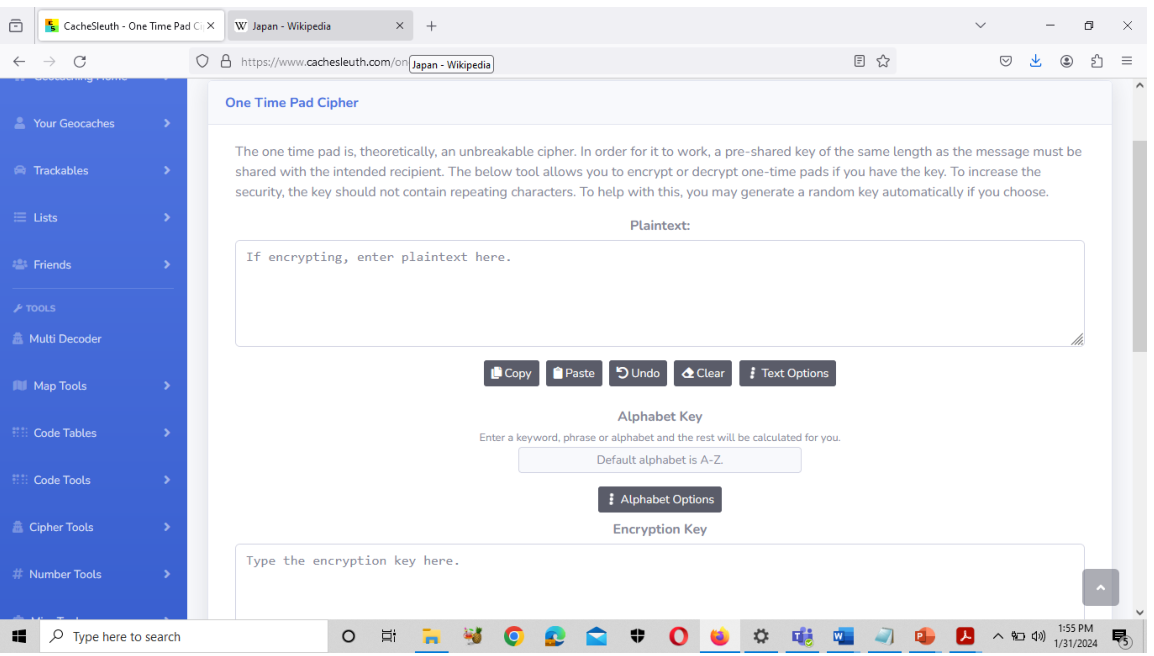
\includegraphics[width=126.21mm,height=180.28mm]{../../images/llm/page_012_img_01.png}%
\end{textblock*}

\end{document}
